\chapter{The latent space model for social influence}\label{ch:influence}

\section{The model}

With \opt{influence(}\emph{outcome lag} [\emph{covariates}]\opt{)} \nwlsm{} fits the latent space model for social influence of Sweet and Adhikari~\cite{sweet2020}: the latent space model of the ties and, jointly with it, a linear model for an actor-level outcome in which social influence acts through the latent positions that are estimated from the network. The variables hold one observation per actor, in the order of the actors of the network: first the outcome $y_t$, measured after the network was formed, second the same outcome $y_{t-1}$ measured before (the lagged outcome), then any other regressors. The outcome of actor $k$ is
\begin{equation}
y_k=\beta_0+\beta_1y_{t-1,k}+\beta_2x_{k2}+\dots+\beta_{\text{influence}}\,m_k+\varepsilon_k,\qquad \varepsilon_k\sim N(0,\sigma_y^2),\qquad m_k=\sum_jw_{kj}\,y_{t-1,j},
\end{equation}
where $m_k$ is the weighted mean of the lagged outcomes of the other actors. The weights depend on the distances between the latent positions: $w_{kj}$ is proportional to $f(\lVert z_k-z_j\rVert)$ over the \opt{neighbors()} actors that are nearest to $k$ in the latent space (all other actors by default) and sums to 1 for each $k$; $f(d)=1/d$ with \opt{weight(invdist)} (the weights of the paper) or $f(d)=\exp(-d)$ with \opt{weight(expdist)}. Actors who are close in the latent space, in practice those with many ties to $k$ or to the same others, are therefore the most influential for $k$; ties to $k$ are not needed to influence $k$. The coefficient $\beta_{\text{influence}}$ is the effect of social influence. The lagged outcome is always a regressor. The weights change with the positions, so the outcome also informs the positions: the network and the outcome parameters are estimated in one MCMC run.

\section{The sampler and the priors}

The positions are updated one actor at a time by random-walk Metropolis--Hastings, whose acceptance ratio contains the change of the log likelihood of the ties and of all outcomes (the weights of the actor who moves, and its weight in the others' means). The outcome coefficients and the error variance are drawn by Gibbs steps given the weights (a normal and an inverse gamma distribution). The priors are $N(0,\texttt{obvar})$ for the outcome coefficients (default variance 100) and an inverse gamma distribution with shape and rate \opt{osigma()} (default 0.01 0.01) for the error variance. The network part (coefficients, effects, clusters, family, priors) is the model of Chapter~\ref{ch:model}. The influence model needs the Euclidean distance and cannot be combined with \opt{bilinear}.

\section{Differences from the paper}

\begin{itemize}[nosep]
  \item The intercept of the tie model is estimated; the paper fixes it at 2 to resolve a weak trade-off with the variance of the positions. The prior of the positions here is that of \latentnet{}, whose scale grows with the number of actors.
  \item The variance of the positions has the \latentnet{} prior instead of an inverse gamma prior.
  \item The outcome coefficients and the error variance are updated by Gibbs steps (the same posterior as random-walk steps), and the default prior of the error variance, inverse gamma(0.01, 0.01), is weaker than the paper's.
  \item Covariates of the ties are allowed; the paper uses none.
  \item One network and one outcome wave are modelled. The hierarchical version for several networks with random coefficients, and the paper's indicator that makes actors without close neighbours immune to influence, are not implemented.
\end{itemize}
Influence needs variation in the lagged outcome among the actors who are weighted: with all other actors as neighbours the weighted means are nearly constant and the influence effect is weakly identified; a moderate \opt{neighbors()} (as in the application of the paper, about the number of ties an actor can name) gives more information, and a \opt{neighbors()} much larger than the true number of influential actors biases the effect.

\section{An example with simulated data}

No data set of the package family has an outcome measured before and after a network was formed, so the example uses simulated data with a known influence effect. Sixty actors have positions in the plane, ties by the latent distance (log odds $1.5-\text{distance}$), a lagged outcome and a covariate, and an outcome $y=0.5+0.6\,y_{t-1}-0.4\,x+1\cdot m+\varepsilon$ with error standard deviation 0.5, where $m$ is the inverse-distance weighted mean of the lagged outcomes of the 8 nearest actors. The true values are therefore known:
\showlog{infl_sim}
The model is fitted with the correct number of neighbours:
\showlog{infl_fit}
The header shows two log likelihoods, that of the ties and that of the outcomes. The table has two equations: the tie model (\texttt{Network (ties)}) and the outcome model, whose last row is the influence effect. The posterior means are close to the true values: the intercept of the ties 1.46 (true 1.5), the outcome intercept 0.45 (0.5), the lagged outcome 0.54 (0.6), the covariate $-0.33$ ($-0.4$), the influence effect 1.15 (1) and the error variance 0.16 (0.25); every true value is inside its 95\% interval. The two chains agree (Gelman--Rubin statistic 1.004 at most).

\texttt{estat influence} summarises the influence effect and the weights:
\showlog{infl_estat}
It shows the outcome equation, the posterior probability that the influence effect is positive, the R-squared of the posterior mean predictions with and without the influence term, the mean effective number of influencing actors (the inverse of the sum of squared weights) and the actors who exert the most influence (the column sums of the posterior mean weights $e(W)$) with the exposure they receive. \opt{predict()}, \opt{exposure()} and \opt{exerted()} store the posterior mean prediction, the exposure $m_k$ and the influence exerted in new variables (one observation per actor); \opt{graph} plots observed against predicted outcomes, and \texttt{nwlsmplot, size(influence)} sizes the actors by the influence they exert. The results are in \texttt{r(influence)}, \texttt{r(influence\_sd)}, \texttt{r(influence\_lower)}, \texttt{r(influence\_upper)}, \texttt{r(prob\_positive)}, \texttt{r(r2)}, \texttt{r(r2\_noinfluence)}, \texttt{r(eff\_neighbors)} and \texttt{r(exerted)}. The chain diagnostics include the outcome coefficients:
\showlog{infl_diag}
\begin{figure}[ht]\centering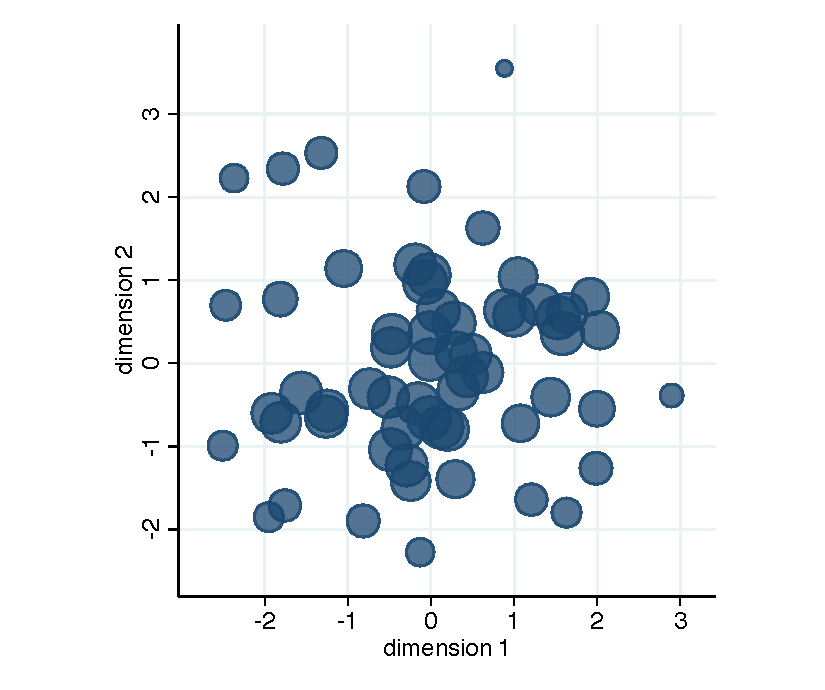
\includegraphics[width=0.85\textwidth]{fig/fig_infl_map.pdf}
\caption{\texttt{nwlsmplot, size(influence)} for the simulated data: actors in the latent space (ties not drawn), sized by the influence they exert on the outcomes of the others.}\end{figure}
\begin{figure}[ht]\centering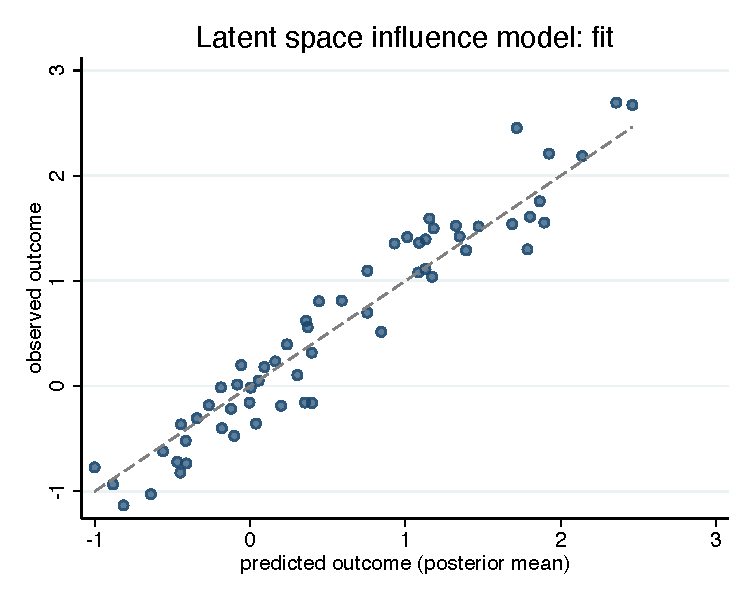
\includegraphics[width=0.7\textwidth]{fig/fig_infl_pred.pdf}
\caption{\texttt{estat influence, graph}: observed and posterior mean predicted outcomes.}\end{figure}

\section{Stored results of the influence model}

\texttt{e(b)} and \texttt{e(V)} hold the posterior means and the covariance of the tie coefficients (equation \texttt{network}) and of the outcome coefficients (equation \texttt{outcome}, the last is the influence effect); \texttt{e(summary)}, \texttt{e(rhat)} and \texttt{estat mcmcdiag} include them, and the error variance is the row \texttt{sigma2\_y} of \texttt{e(vsummary)}. \texttt{e(W)} is the posterior mean weight matrix (row $k$: the weights of the actors on $k$), \texttt{e(pred)} holds for each actor the outcome, the posterior mean predicted outcome, the exposure $m_k$ and the part of the prediction due to influence, and \texttt{e(prob\_positive)} is the posterior probability that the influence effect is positive. The macros \texttt{e(influence)}, \texttt{e(outcome)}, \texttt{e(lagvar)}, \texttt{e(ocovariates)}, \texttt{e(weight)} and the scalars \texttt{e(neighbors)}, \texttt{e(obvar)}, \texttt{e(osigma\_a)}, \texttt{e(osigma\_b)}, \texttt{e(ll\_outcome)} describe the model. With \opt{savedraws()} the draws of the outcome coefficients are saved with the other draws.
